%!TEX root=../document.tex

\section{Ergebnisse}
\subsection{view}
Die Klasse \verb|view.py| wurde automatisch von PySide erstellt. In dieser Klasse wurde bereits automatisch auf den close-button das Signal der \verb|close()| Methode gelegt. 
Generell ist zu sagen, dass diese Klasse nicht weiter verändert werden soll.

\begin{minipage}{\linewidth}
	\centering
	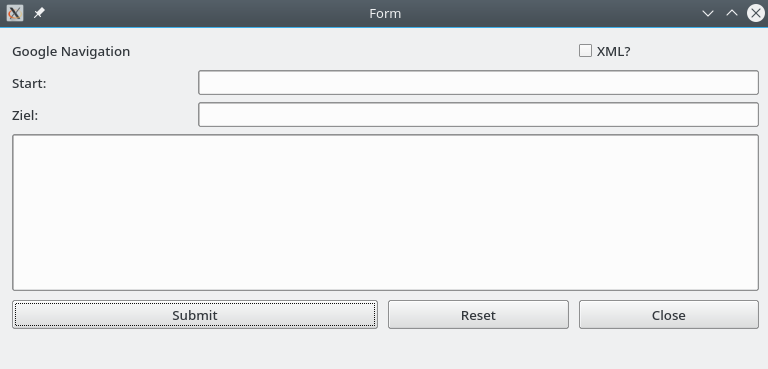
\includegraphics[width=0.8\linewidth]{images/gui}
	\figcaption{Layout der View}
\end{minipage}

\begin{lstlisting}[language=python]
class Ui_Form(object):
	def setupUi(self, Form):
		Form.setObjectName("Form")
		Form.resize(769, 339)
		self.gridLayout = QtGui.QGridLayout(Form)
		self.gridLayout.setObjectName("gridLayout")
		self.output_ok = QtGui.QLabel(Form)
		self.output_ok.setText("")
		self.output_ok.setObjectName("output_ok")
		self.gridLayout.addWidget(self.output_ok, 5, 0, 1, 1)
		self.button_submit = QtGui.QPushButton(Form)
		self.button_submit.setObjectName("button_submit")
		self.gridLayout.addWidget(self.button_submit, 4, 0, 1, 2)
		self.button_reset = QtGui.QPushButton(Form)
		self.button_reset.setObjectName("button_reset")
		self.gridLayout.addWidget(self.button_reset, 4, 2, 1, 1)
		self.label_3 = QtGui.QLabel(Form)
		self.label_3.setObjectName("label_3")
		self.gridLayout.addWidget(self.label_3, 2, 0, 1, 1)
		self.label_2 = QtGui.QLabel(Form)
		self.label_2.setObjectName("label_2")
		self.gridLayout.addWidget(self.label_2, 1, 0, 1, 1)
		self.input_ziel = QtGui.QLineEdit(Form)
		self.input_ziel.setObjectName("input_ziel")
		self.gridLayout.addWidget(self.input_ziel, 2, 1, 1, 3)
		self.label = QtGui.QLabel(Form)
		self.label.setObjectName("label")
		self.gridLayout.addWidget(self.label, 0, 0, 1, 2)
		self.button_close = QtGui.QPushButton(Form)
		self.button_close.setObjectName("button_close")
		self.gridLayout.addWidget(self.button_close, 4, 3, 1, 1)
		self.input_start = QtGui.QLineEdit(Form)
		self.input_start.setObjectName("input_start")
		self.gridLayout.addWidget(self.input_start, 1, 1, 1, 3)
		self.output = QtGui.QTextBrowser(Form)
		self.output.setObjectName("output")
		self.gridLayout.addWidget(self.output, 3, 0, 1, 4)
		self.mode = QtGui.QCheckBox(Form)
		self.mode.setObjectName("mode")
		self.gridLayout.addWidget(self.mode, 0, 3, 1, 1)
		
		self.retranslateUi(Form)
		QtCore.QObject.connect(self.button_close, QtCore.SIGNAL("clicked()"), Form.close)
		QtCore.QMetaObject.connectSlotsByName(Form)
		
	def retranslateUi(self, Form):
		Form.setWindowTitle(QtGui.QApplication.translate("Form", "Form", None, QtGui.QApplication.UnicodeUTF8))
		self.button_submit.setText(QtGui.QApplication.translate("Form", "Submit", None, QtGui.QApplication.UnicodeUTF8))
		self.button_reset.setText(QtGui.QApplication.translate("Form", "Reset", None, QtGui.QApplication.UnicodeUTF8))
		self.label_3.setText(QtGui.QApplication.translate("Form", "Ziel:", None, QtGui.QApplication.UnicodeUTF8))
		self.label_2.setText(QtGui.QApplication.translate("Form", "Start:", None, QtGui.QApplication.UnicodeUTF8))
		self.label.setText(QtGui.QApplication.translate("Form", "Google Navigation", None, QtGui.QApplication.UnicodeUTF8))
		self.button_close.setText(QtGui.QApplication.translate("Form", "Close", None, QtGui.QApplication.UnicodeUTF8))
		self.mode.setText(QtGui.QApplication.translate("Form", "XML?", None, QtGui.QApplication.UnicodeUTF8))


\end{lstlisting}

\subsection{controller}
In dieser Klasse wird das \verb|QWidget| initialisiert, indem der \verb|controller| selber ein \verb|QWidget| darstellt indem er davon erbt. Es wird die GUI dem \verb|QWidget| hinzugfeügt und gestartet. Im \verb|controller| gibt es 3 Methoden:

\subsubsection{init()}
Dadurch dass der controller von QWidget erbt, muss natürlich zuerst der Superkonstruktor aufgerufen werden. Anschließend wird ein Objekt von der view klasse erzeugt, welches mit \verb|.setupUi()| ''gestartet'' wird.
Es wird noch ein Objektattribut mit einem Objekt vom Model gesetzt, und anschließend werden dem \verb|button_submit| und dem \verb|button_reset| 2 Methoden mit \verb|connect()| hinzugefügt, und zwar \verb|self.submit| und \verb|self.reset|. Wichtig: Keine Klammern da es sich um einen sogenannten \textbf{callback} handelt.

\begin{lstlisting}[language=python]
def __init__(self):
	"""
	When the controller gets initialized, the GUI gets set up, a model member is set and the buttons are connected
	to the respective functions
	
	Important: The Signal on the close Button which closes the windows already got connected
	to the close() slot in the QT-Designer:
	'QtCore.QObject.connect(self.button_close, QtCore.SIGNAL("clicked()"), Form.close)
	QtCore.QMetaObject.connectSlotsByName(Form)'
	"""
	QWidget.__init__(self)
	self.view = view.Ui_Form()
	self.view.setupUi(self)
	self.model = model.Model()
	self.view.button_submit.clicked.connect(self.submit)
	self.view.button_reset.clicked.connect(self.reset)
\end{lstlisting}

\subsubsection{submit()}
Ruft lediglich die \verb|get_route| Methode des Models auf und setzt das GUI Element der View auf den output dieser Methode

\begin{lstlisting}[language=python]
def submit(self):
	"""
	This method gets called when the Submit button gets pressed
	
	The get_route function from the model gets called, which returns the route and a status
	:return: None
	"""
	# get_route gets called with the route-start, route-destionation and a paremeter which
	# determines whether the query should be done via XML or JSON
	route = self.model.get_route(self.view.input_start.text(), self.view.input_ziel.text(), self.view.mode.isChecked())
	self.view.output.setText(route[0])
	self.view.output_ok.setText(route[1])
\end{lstlisting}


\subsubsection{reset()}
Setzt alle Felder auf ihren Ursprungswert zurück.

\begin{lstlisting}[language=python]
def reset(self):
	"""
	Gets called when the reset button is pressed
	
	Sets all input and output fields to empty strings and unchecks the box
	:return:
	"""
	self.view.output.setText("")
	self.view.input_ziel.setText("")
	self.view.input_start.setText("")
	self.view.output_ok.setText("")
	self.view.mode.setChecked(False)
\end{lstlisting}

\subsection{model}
In dieser Klasse wird nun auf die tatsächliche API zugegriffen.
Sie besteht lediglich aus der \verb|get_route()| Methode, da es keine Objektattribute gibt

\subsubsection{get\_route()}
Die Methode hat 3 Parameter: \verb|start|, \verb|destination| und \verb|is_xml|. Der Parameter \verb|is_xml| ist ein boolean, und ist dann true sobald eine xml Anfrage statt einer JSON anfrage gestellt werden soll.

Ob XML oder JSON, zuerst wird mit \verb|requests.get()| die API aufgerufen und man bekommt eine \verb|response| zurück. Diese response kann nun in die jeweilige Datenstruktur gebracht werden, und es kann ein String geformt werden welcher zurückgegeben wird. Wichtig ist, dass an ein GUI-Element zurückgegeben wird welches HTML verarbeiten kann, dadurch können Dinge fett geschrieben werden mit \textbf{<b>}.

\begin{lstlisting}[language=python]
def get_route(self, start, destination, is_xml):
	"""
	Creates a query to the google drive API, either parses the XML or JSON File
	:param start: the string which holds the information where the route is to be started
	:param destination: the string which holds the information where the route ends
	:param is_xml: boolean which determines whether a XML or JSON file is to be requested
	:return: A html-formatted string where the route is described and a status for the GUI
	"""
	output = ""
	if is_xml:
		# GET is used because no information is posted, only received
		# important: the parameter mode=driving and language=de might seem unnecessary, but its important
		# that these are at the beginning to prevent injection-strings, for example 'Jaegerstrasse&mode=walking'
		response = requests.get(
		url="https://maps.googleapis.com/maps/api/directions/xml?mode=driving&language=de&origin=%s&destination=%s" % (
		start, destination))
		# get the root element of the XML structure
		xml_data = ET.fromstring(response.text)
		# get the status, which is the first child element
		status = xml_data[0].text
		# check for certain statuses, and return if certain where returned
		if status == 'NOT_FOUND' or status == 'INVALID_REQUEST' or status == 'ZERO_RESULTS':
			return [output, "Es wurde der Status %s zurueckgegeben, Eingabe ueberpruefen!" % (status)]
		else:
			status_ok = "Berechnung Ok!"
		
		# get the legend
		leg = xml_data[1][1]
		# from the legend extract the information how long the trip is in duration and distance
		output += "<p>Die Gesamtdauer betraegt <b>%s</b>, die Gesamtentfernung: <b>%s</b> </p>" % (
		leg.find('duration')[1].text, leg.find('distance')[1].text)
		
		# iterate through all steps in the legend
		for step in leg.findall('step'):
			# append the html_instruction, distance and duration information to the output string
			output += "%s, Entfernung %s, Dauer %s <br>" % (
			step.find('html_instructions').text, step.find('distance')[1].text, step.find('duration')[1].text)
		# return the route information and the status
		return [output, status_ok]
	else:
		# request json response
		response = requests.get(
		url="https://maps.googleapis.com/maps/api/directions/json?mode=driving&language=de&origin=%s&destination=%s" % (
		start, destination))
		# the requests module is able to convert json into a dictionary which is more easy to work with
		json_data = response.json()
		status = json_data["status"]
		# again check for certain statuses and return if a bad one was returned
		if status == 'NOT_FOUND' or status == 'INVALID_REQUEST' or status == 'ZERO_RESULTS':
			return [output, "Es wurde der Status %s zurueckgegeben, Eingabe ueberpruefen!" % (status)]
		else:
			status_ok = "Berechnung Ok!"
		
		# get the legend information
		legs = json_data["routes"][0]["legs"][0]
		# get all steps
		steps = legs["steps"]
		# also extract the total duration and distance for the route from the legend
		output += "<p>Die Gesamtdauer betraegt <b>%s</b>, die Gesamtentfernung: <b>%s</b> </p>" % (legs["duration"]["text"], legs["distance"]["text"])
		
		# iterate through the steps
		for step in steps:
			# append the html_instructions, distance and duration to the output string
			output += "%s, Entfernung %s, Dauer %s <br>" % (step["html_instructions"], step["distance"]["text"], step["duration"]["text"])
		# return the route string and the status
		return [output, status_ok]
\end{lstlisting}

\subsection{run}
Diese Klasse startet die Application und das Widget

\begin{lstlisting}[language=python]
if __name__ == '__main__':
	app = QApplication(sys.argv)
	c = controller.Controller()
	c.show()
	
	sys.exit(app.exec_())

\end{lstlisting}